\documentclass[11pt,a4paper]{article}

% Packages
\usepackage[utf8]{inputenc}
\usepackage[T1]{fontenc}
\usepackage{graphicx}
\usepackage{amsmath}
\usepackage{amssymb}
\usepackage{booktabs}
\usepackage{hyperref}
\usepackage{cleveref}
\usepackage{float}
\usepackage{listings}
\usepackage{xcolor}
\usepackage[margin=2.5cm]{geometry}
\usepackage{caption}
\usepackage{subcaption}
\usepackage{tikz}
\usepackage{siunitx}
\usepackage{bytefield}

% TikZ libraries
\usetikzlibrary{shapes,arrows,positioning,calc,patterns,decorations.pathreplacing}

% Code listing style
\lstset{
    basicstyle=\ttfamily\small,
    keywordstyle=\color{blue},
    commentstyle=\color{green!60!black},
    stringstyle=\color{red},
    numbers=left,
    numberstyle=\tiny\color{gray},
    breaklines=true,
    frame=single
}

% Better spacing
\setlength{\parskip}{0.6em}
\renewcommand{\arraystretch}{1.3}

\title{Analysis of the Interest and Impact of a Hybrid FP16/FP32 Real-Time Graphics Pipeline:\\
Implementation, Performance and Image Quality Metrics Assessment}

\author{Stanis KAPUSTA}

\begin{document}

    \maketitle

    \begin{abstract}
        Real-time graphics applications constantly seek optimization opportunities to achieve better performance while maintaining visual quality. This paper investigates the potential of hybrid precision rendering, where selected pipeline stages use 16-bit floating-point (FP16) instead of the traditional 32-bit format (FP32). The fundamentals of floating-point representation are first reviewed, followed by an examination of the current state of mixed precision techniques in the graphics industry. Emerging technologies such as cooperative vectors are then analyzed along with their limitations in traditional rendering architectures. Through a case study on Screen-Space Ambient Occlusion (SSAO), performance gains, memory savings, and visual quality trade-offs of FP16 adoption are evaluated. The results demonstrate that a 41\% performance improvement and 23.5\% memory reduction can be achieved with imperceptible quality loss (PSNR 63 dB, SSIM 0.9998), providing practical guidelines for developers considering hybrid precision in their rendering pipelines.
    \end{abstract}

% ============================================================================
    \section{Introduction}
    \label{sec:introduction}
% ============================================================================

    Real-time computer graphics has evolved considerably over the past decades. Modern applications such as video games, virtual reality, and interactive simulations demand increasingly complex visual effects while maintaining high frame rates. This constant push for better performance has led developers to explore various optimization strategies, from algorithmic improvements to hardware-specific techniques.

    One area that has received renewed attention is numerical precision. Traditionally, graphics pipelines have relied on 32-bit floating-point (FP32) arithmetic for most calculations. This format offers a good balance between range, precision, and performance for general-purpose computing. However, not all stages of a rendering pipeline require the full precision that FP32 provides. In many cases, intermediate calculations or stored values could use reduced precision without any visible impact on the final image.

    The 16-bit floating-point format (FP16) presents an interesting alternative. With half the memory footprint of FP32, it can reduce memory bandwidth requirements and potentially improve cache efficiency. On modern GPU architectures, FP16 operations can also be executed faster than their FP32 counterparts, sometimes at twice the throughput. These benefits make hybrid precision pipelines---where FP16 and FP32 are used selectively based on the requirements of each stage---an attractive optimization target.

    However, adopting FP16 is not without risks. The reduced precision and range can introduce visual artifacts in certain scenarios, particularly when dealing with large coordinate spaces or subtle color gradations. Understanding where FP16 can be safely applied, and where it cannot, is essential for making informed optimization decisions.

    This paper investigates the practical benefits and limitations of hybrid FP16/FP32 precision in real-time rendering, addressing three key questions: what performance and memory gains can be expected from FP16 adoption, under what conditions reduced precision leads to visible quality degradation, and which rendering techniques are good candidates for hybrid precision optimization.

    The paper is organized as follows. Section~\ref{sec:floating-point} reviews the fundamentals of floating-point representation, explaining the differences between FP32 and FP16. Section~\ref{sec:state-of-art} examines the current state of mixed precision techniques in the graphics industry. Section~\ref{sec:cooperative-vectors} discusses emerging technologies like cooperative vectors and their applicability to traditional rendering. Section~\ref{sec:methodology} describes the experimental methodology used in this study. Section~\ref{sec:case-studies} presents detailed case studies with performance measurements and quality assessments. Finally, Section~\ref{sec:discussion} analyzes the results and provides practical guidelines, followed by conclusions in Section~\ref{sec:conclusion}.

% ============================================================================
    \section{Floating-Point Representation}
    \label{sec:floating-point}
% ============================================================================

    \subsection{The IEEE 754 Standard}
    \label{subsec:ieee754}

    The IEEE 754 standard~\cite{ieee754} defines the representation and behavior of floating-point numbers in modern computing systems. First published in 1985 and revised in 2008 and 2019, it provides a consistent framework for representing real numbers with finite precision across different hardware platforms.

    A floating-point number under IEEE 754 consists of three components:
    \begin{itemize}
        \item A \textbf{sign bit} indicating whether the number is positive or negative
        \item An \textbf{exponent field} representing the power of two by which the significand is scaled
        \item A \textbf{significand} (or mantissa) containing the fractional component with an implicit leading 1 for normalized numbers
    \end{itemize}

    The value of a normalized floating-point number is computed as:
    \begin{equation}
        \text{value} = (-1)^s \times 2^{E - \text{bias}} \times (1 + M)
    \end{equation}
    where $s$ is the sign bit, $E$ is the stored exponent, and $M$ is the fractional part of the mantissa. The bias is a constant that allows both positive and negative exponents to be stored in an unsigned field.

    The standard also defines special values to handle exceptional cases:
    \begin{itemize}
        \item \textbf{Zero:} Both exponent and mantissa are zero (signed zeros $+0$ and $-0$ exist)
        \item \textbf{Infinity ($\pm\infty$):} All-ones exponent with zero mantissa
        \item \textbf{NaN:} All-ones exponent with non-zero mantissa
        \item \textbf{Denormalized:} Zero exponent with non-zero mantissa (enables gradual underflow)
    \end{itemize}

    \subsection{FP32 and FP16: Precision, Range and Trade-offs}
    \label{subsec:fp32-fp16}

    The two formats of primary interest for graphics applications are single precision (FP32, also called \texttt{float}) and half precision (FP16, also called \texttt{half}). Figure~\ref{fig:fp-formats} illustrates the bit allocation for both formats.

    \begin{figure}[H]
        \centering
        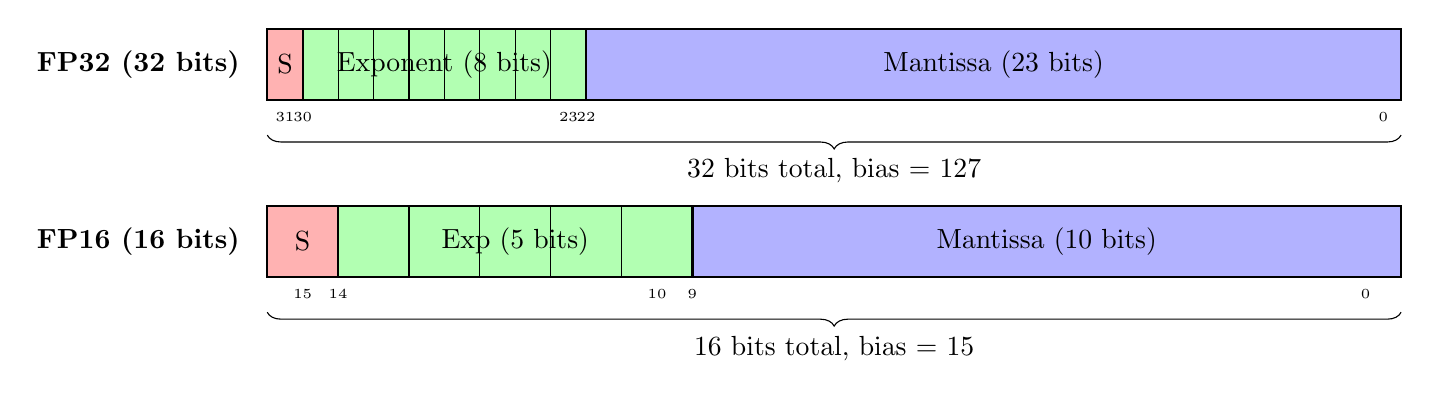
\begin{tikzpicture}[scale=0.45]
            % FP32 format
            \node[anchor=east] at (-0.5, 1) {\textbf{FP32 (32 bits)}};

            % Sign bit
            \fill[red!30] (0,0) rectangle (1,2);
            \draw[thick] (0,0) rectangle (1,2);
            \node at (0.5,1) {S};
            \node[font=\tiny] at (0.5,-0.5) {31};

            % Exponent (8 bits)
            \fill[green!30] (1,0) rectangle (9,2);
            \draw[thick] (1,0) rectangle (9,2);
            \foreach \x in {2,3,4,5,6,7,8} \draw (\x,0) -- (\x,2);
            \node at (5,1) {Exponent (8 bits)};
            \node[font=\tiny] at (1,-0.5) {30};
            \node[font=\tiny] at (8.5,-0.5) {23};

            % Mantissa (23 bits)
            \fill[blue!30] (9,0) rectangle (32,2);
            \draw[thick] (9,0) rectangle (32,2);
            \node at (20.5,1) {Mantissa (23 bits)};
            \node[font=\tiny] at (9,-0.5) {22};
            \node[font=\tiny] at (31.5,-0.5) {0};

            % Brace for total
            \draw[decorate,decoration={brace,amplitude=5pt,mirror}] (0,-1) -- (32,-1)
            node[midway,below=5pt] {32 bits total, bias = 127};

            % FP16 format
            \node[anchor=east] at (-0.5, -4) {\textbf{FP16 (16 bits)}};

            % Sign bit
            \fill[red!30] (0,-5) rectangle (2,-3);
            \draw[thick] (0,-5) rectangle (2,-3);
            \node at (1,-4) {S};
            \node[font=\tiny] at (1,-5.5) {15};

            % Exponent (5 bits)
            \fill[green!30] (2,-5) rectangle (12,-3);
            \draw[thick] (2,-5) rectangle (12,-3);
            \foreach \x in {4,6,8,10} \draw (\x,-5) -- (\x,-3);
            \node at (7,-4) {Exp (5 bits)};
            \node[font=\tiny] at (2,-5.5) {14};
            \node[font=\tiny] at (11,-5.5) {10};

            % Mantissa (10 bits)
            \fill[blue!30] (12,-5) rectangle (32,-3);
            \draw[thick] (12,-5) rectangle (32,-3);
            \node at (22,-4) {Mantissa (10 bits)};
            \node[font=\tiny] at (12,-5.5) {9};
            \node[font=\tiny] at (31,-5.5) {0};

            % Brace for total
            \draw[decorate,decoration={brace,amplitude=5pt,mirror}] (0,-6) -- (32,-6)
            node[midway,below=5pt] {16 bits total, bias = 15};
        \end{tikzpicture}
        \caption{Bit layout comparison of IEEE 754 FP32 and FP16 formats. The sign bit (S) occupies the most significant position, followed by the exponent field, and finally the mantissa in the least significant bits.}
        \label{fig:fp-formats}
    \end{figure}

    FP32 uses 32 bits with an 8-bit exponent (bias of 127) and a 23-bit mantissa, providing approximately 7 decimal digits of precision ($2^{24} \approx 16.7$ million distinct values per power of two) and a range from approximately $1.18 \times 10^{-38}$ to $3.4 \times 10^{38}$. This format has been the default for graphics programming since the transition from fixed-point arithmetic in the early 2000s.

    FP16, in contrast, uses only 16 bits with a 5-bit exponent (bias of 15) and a 10-bit mantissa. This provides approximately 3.3 decimal digits of precision ($2^{11} = 2048$ distinct values per power of two, including the implicit leading 1) and a considerably smaller range from approximately $6.1 \times 10^{-5}$ to $65,504$. Table~\ref{tab:fp-comparison} summarizes the key differences.

    \begin{table}[H]
        \centering
        \caption{Comparison of IEEE 754 floating-point formats relevant to graphics}
        \label{tab:fp-comparison}
        \begin{tabular}{lccccc}
            \toprule
            \textbf{Format} & \textbf{Total} & \textbf{Exponent} & \textbf{Mantissa} & \textbf{Range} & \textbf{Precision} \\
            \midrule
            FP32 & 32 bits & 8 bits & 23 bits & $\pm 3.4 \times 10^{38}$ & $\sim$7 digits \\
            FP16 & 16 bits & 5 bits & 10 bits & $\pm 65,504$ & $\sim$3.3 digits \\
            BF16 & 16 bits & 8 bits & 7 bits & $\pm 3.4 \times 10^{38}$ & $\sim$2 digits \\
            \bottomrule
        \end{tabular}
    \end{table}

    The limited range and precision of FP16 have important implications for graphics applications:
    \begin{itemize}
        \item Values below $6.1 \times 10^{-5}$ become denormalized or zero, potentially causing ``black crush'' in dark image regions
        \item Values above 65,504 overflow to infinity, problematic for HDR rendering or large world coordinates
        \item The 3.3 decimal digits of precision can cause visible banding in smooth color gradients
    \end{itemize}

    \subsection{Precision Distribution}
    \label{subsec:precision-dist}

    An important property of floating-point representation is that precision is relative, not absolute. The representable values are more densely packed near zero and become sparser as magnitude increases. Figure~\ref{fig:precision-dist} visualizes this non-uniform distribution for FP16.

    \begin{figure}[H]
        \centering
        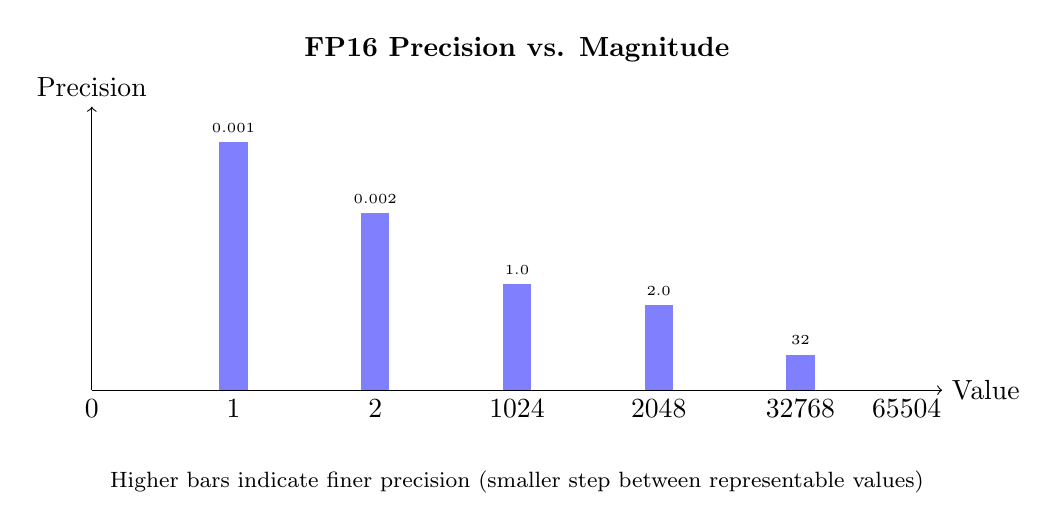
\begin{tikzpicture}[scale=0.9]
            % Axis
            \draw[->] (0,0) -- (12,0) node[right] {Value};
            \draw[->] (0,0) -- (0,4) node[above] {Precision};

            % Labels on x-axis
            \node[below] at (0,0) {0};
            \node[below] at (2,0) {1};
            \node[below] at (4,0) {2};
            \node[below] at (6,0) {1024};
            \node[below] at (8,0) {2048};
            \node[below] at (10,0) {32768};
            \node[below] at (11.5,0) {65504};

            % Precision levels (inverted - higher bar = finer precision)
            \fill[blue!50] (1.8,0) rectangle (2.2,3.5);
            \node[above,font=\tiny] at (2,3.5) {0.001};

            \fill[blue!50] (3.8,0) rectangle (4.2,2.5);
            \node[above,font=\tiny] at (4,2.5) {0.002};

            \fill[blue!50] (5.8,0) rectangle (6.2,1.5);
            \node[above,font=\tiny] at (6,1.5) {1.0};

            \fill[blue!50] (7.8,0) rectangle (8.2,1.2);
            \node[above,font=\tiny] at (8,1.2) {2.0};

            \fill[blue!50] (9.8,0) rectangle (10.2,0.5);
            \node[above,font=\tiny] at (10,0.5) {32};

            % Title
            \node[above] at (6,4.5) {\textbf{FP16 Precision vs. Magnitude}};
            \node[below] at (6,-1) {\footnotesize Higher bars indicate finer precision (smaller step between representable values)};
        \end{tikzpicture}
        \caption{FP16 precision decreases as value magnitude increases. Between 1 and 2, there are 1024 distinct representable values with precision of approximately 0.001. Between 32768 and 65504, the same 1024 values must span a much larger range, yielding precision of only 32.}
        \label{fig:precision-dist}
    \end{figure}

    This non-uniform distribution is particularly relevant when storing world-space positions. A scene spanning 1000 units would have centimeter-level precision near the origin but only meter-level precision at the boundaries when using FP16. For this reason, view-space coordinates (which are typically bounded to a smaller range near the camera) are often more suitable for FP16 storage than world-space coordinates.

    The BF16 (Brain Float 16) format, included in Table~\ref{tab:fp-comparison} for reference, represents an alternative approach that trades mantissa bits for exponent bits. With 8 exponent bits (matching FP32) but only 7 mantissa bits, BF16 maintains the same dynamic range as FP32 while sacrificing precision. This format was developed primarily for machine learning applications where range matters more than precision, but its poor precision of approximately 2 decimal digits makes it less suitable for graphics applications where subtle color variations are important~\cite{fp16-wiki}.

% ============================================================================
    \section{State of the Art: Mixed Precision in Real-Time Graphics}
    \label{sec:state-of-art}
% ============================================================================

    \subsection{Historical Context}
    \label{subsec:history}

    The use of reduced precision in graphics has a cyclical history~\cite{mjp-fp16}. During the DirectX 9 era from 2002 to 2006, FP16 was an important optimization on NVIDIA's GeForce FX, 6-series, and 7-series hardware. The \texttt{half} type in Cg and HLSL allowed developers to explicitly request 16-bit operations, and careful use could yield significant performance improvements on those architectures.

    The transition to DirectX 10 and unified shader architectures marked a shift away from FP16. The hardware moved toward executing all shader operations at full FP32 precision, and the \texttt{half} type was silently promoted to \texttt{float} by compilers. For nearly a decade, FP16 became largely irrelevant in real-time graphics programming.

    Interest in FP16 resurged around 2016--2018 with the introduction of dedicated half-precision hardware in modern GPU architectures. This revival was initially driven by machine learning workloads, where reduced precision training proved viable, but graphics applications could also benefit from the new capabilities. NVIDIA's Turing architecture (RTX 20 series, 2018) and AMD's Vega (2017) and RDNA architectures reintroduced efficient FP16 execution paths, making hybrid precision pipelines practical once again.

    \subsection{Current Hardware Support}
    \label{subsec:hardware}

    Modern GPUs offer varying levels of FP16 support, with important distinctions between vendors and product lines that developers must understand when targeting hybrid precision.

    \textbf{NVIDIA's} support for FP16 varies significantly by GPU tier. Their Tensor Cores, available on Turing (RTX 20 series) and later architectures, can perform matrix operations at FP16 with extremely high throughput---the RTX 4090 achieves approximately 330 TFLOPS for FP16 tensor operations compared to 82 TFLOPS for FP32 shader operations~\cite{nvidia-tensor}.

    However, standard shader cores on GeForce consumer cards typically execute FP16 at the same rate as FP32, meaning there is no direct throughput benefit from FP16 arithmetic. The performance advantage on these cards comes instead from reduced register pressure improving occupancy and from reduced memory bandwidth. Professional Quadro cards often provide 2:1 FP16:FP32 throughput ratios even in standard shader cores.

    \textbf{AMD's} RDNA architecture provides more consistent FP16 benefits across their product line. RDNA can execute two FP16 operations in the time of one FP32 operation using packed math instructions, making the throughput benefit available on consumer Radeon cards. RDNA 3 further introduced Wave Matrix Multiply Accumulate (WMMA) instructions for accelerated matrix operations.

    \textbf{Intel's} integrated and discrete GPUs from Gen9 through Xe architectures report FP16 capability, though actual performance benefits vary by generation and workload.

    \textbf{Mobile GPUs} from ARM (Mali) and Qualcomm (Adreno) have historically provided strong FP16 support, as power efficiency is paramount on battery-powered devices.

    \subsection{Implementation Approaches}
    \label{subsec:approaches}

    There are two distinct approaches to using FP16 in shaders, each with different trade-offs~\cite{mjp-fp16}:

    \textbf{Flexible precision} uses types such as \texttt{min16float} in HLSL or \texttt{mediump} in GLSL, which provide a hint to the compiler that reduced precision is acceptable. The compiler and driver may or may not use FP16 based on target hardware. This approach is portable but types cannot be used for buffer storage and require explicit casting from FP32.

    \textbf{Explicit FP16} uses types like \texttt{half} or \texttt{float16\_t} that guarantee 16-bit execution on supported hardware. In HLSL, this requires the DXC compiler with \texttt{-enable-16bit-types} and Shader Model 6.2+. This allows FP16 storage in buffers directly, but requires capability checking and may need separate shader variants for older hardware.

    \textbf{Vulkan requirements:} Explicit FP16 support requires two extensions:
    \begin{itemize}
        \item \texttt{VK\_KHR\_shader\_float16\_int8} enables arithmetic operations
        \item \texttt{VK\_KHR\_16bit\_storage} provides buffer access flags
    \end{itemize}
    Not all combinations are universally supported---NVIDIA Turing lacks \texttt{storageInputOutput16} while AMD lacks \texttt{storagePushConstant16}~\cite{mjp-fp16}.

% ============================================================================
    \section{Emerging Technologies: Cooperative Vectors}
    \label{sec:cooperative-vectors}
% ============================================================================

    \subsection{Cooperative Matrix Operations}
    \label{subsec:coop-matrix}

    The \texttt{VK\_KHR\_cooperative\_matrix} extension~\cite{vk-coop-matrix} represents a significant advancement in GPU compute capabilities by exposing hardware-accelerated matrix multiplication operations that leverage dedicated tensor cores or similar fixed-function units. Originally introduced as an NVIDIA-specific extension (\texttt{VK\_NV\_cooperative\_matrix}) and later promoted to a cross-vendor Khronos standard, cooperative matrices enable the classic deep learning operation $D = A \times B + C$ to execute at throughputs far exceeding traditional shader arithmetic.

    The fundamental principle behind cooperative matrices is that multiple shader invocations within a subgroup cooperatively own and operate on matrix data. Rather than each thread processing independent data, the threads collectively load, multiply, and store matrices using an opaque, implementation-defined data layout. This allows GPU vendors to optimize the matrix multiply operator in ways that best suit their hardware---whether through dedicated tensor cores, specialized ALU configurations, or optimized memory access patterns---while presenting a unified API to developers~\cite{nvidia-coop-matrix}.

    Hardware support for cooperative matrices has expanded considerably since their introduction. NVIDIA Turing and later architectures support the extension through their tensor cores, with driver support shipping since 2019. AMD's RADV driver exposes cooperative matrices on RDNA 3 (GFX11) hardware using Wave Matrix Multiply Accumulate instructions, with support merged into Mesa 23.3. Select mobile GPUs from Qualcomm also provide support, though with varying tile sizes---Adreno Gen5 uses 64$\times$64$\times$16 tiles compared to NVIDIA's typical 16$\times$16$\times$16.

    \subsection{Cooperative Vectors for Neural Networks in Shaders}
    \label{subsec:coop-vectors}

    While cooperative matrices excel at large-scale matrix multiplication, several modern rendering techniques have emerged that require a different computational pattern: independently evaluating small neural networks within each shader invocation. Techniques such as Neural Radiance Caching~\cite{nrc-nvidia}, neural texture compression~\cite{nvidia-neural-rendering}, and neural material models involve having each pixel or ray independently evaluate a multi-layer perceptron (MLP) to predict lighting, decode compressed data, or compute material properties.

    These techniques can benefit from the same dedicated matrix multiply hardware used for cooperative matrices, but they need to work within the standard SIMT (Single Instruction, Multiple Thread) shader programming model rather than the subgroup-wide cooperative model. This mismatch led NVIDIA to develop the \texttt{VK\_NV\_cooperative\_vector} extension~\cite{vk-coop-vector}, which provides a middle ground between full cooperative matrices and traditional scalar operations.

    Unlike cooperative matrix types where data is distributed across many threads, a cooperative vector variable is logically stored in the invocation it belongs to~\cite{vk-coop-vector}. This means each invocation can reference distinct weight matrices, there is no requirement for uniform control flow or fully occupied subgroups (though these conditions improve performance), and the programming model remains familiar to graphics developers. The primary operation is matrix-vector multiplication with bias addition: given a matrix $\mathbf{W}$ of size $M \times K$, an input vector $\mathbf{x}$ of length $K$, and a bias vector $\mathbf{b}$, the operation computes $\mathbf{y} = \mathbf{W}\mathbf{x} + \mathbf{b}$---exactly the affine transformation at the heart of neural network layers.

    The practical benefits of cooperative vectors in production are already visible. NVIDIA's Neural Texture Compression (NTC) technology, which uses cooperative vectors to decode neural-compressed textures at runtime, achieves approximately 80$\times$ texture footprint reduction compared to uncompressed data~\cite{nvidia-neural-rendering}. In one production example, a dragon model requiring over 100 8K UDIM textures was compressed to fit within a 3GB budget on a 16GB GPU---a compression ratio that would be impossible with traditional formats like BC7.

    Microsoft has announced that cooperative vector support is coming to DirectX through collaboration with NVIDIA, AMD, Intel, and Qualcomm~\cite{dx-coop-vector}, signaling industry-wide adoption of this capability for neural rendering techniques.

    \subsection{Limitations in Traditional Rendering}
    \label{subsec:coop-limitations}

    Despite their impressive capabilities, cooperative matrices and vectors have limited applicability to traditional rendering pipelines that do not incorporate neural network evaluation. The fundamental issue is a workload mismatch: traditional rendering operations rarely involve the large, regular matrix multiplications that tensor hardware excels at. Vertex transformation is a 4$\times$4 matrix times a 4-component vector---far too small for cooperative matrices to provide benefit. Lighting calculations involve dot products and simple vector operations. Texture sampling is memory-bound with irregular access patterns that cannot be expressed as matrix multiplication.

    Cooperative matrices also require uniform control flow within subgroups, but traditional shaders often have divergent execution paths. Early fragment culling creates partially occupied subgroups, branching based on material properties causes divergence, and alpha testing with dynamic loops varies per-invocation. The opaque, implementation-defined layout of cooperative matrices is likewise incompatible with standard graphics resources: textures use fixed formats like R8G8B8A8 or BC7, vertex buffers have interleaved attribute layouts, and uniform buffers follow std140/std430 packing rules.

    For traditional graphics optimization that does not involve neural network inference, the simpler approach of using FP16 texture formats and shader precision hints remains more practical than cooperative matrix operations. The benefits of tensor hardware are best realized in dedicated compute passes for post-process neural filters (such as DLSS or FSR with ML components), offline neural network inference, and custom ML-based rendering techniques. This paper therefore focuses on the more broadly applicable technique of hybrid FP16/FP32 precision in conventional rendering passes.

% ============================================================================
    \section{Methodology}
    \label{sec:methodology}
% ============================================================================

    \subsection{Test Framework}
    \label{subsec:framework}

    The experiments in this paper use the Sascha Willems Vulkan Examples~\cite{vk-examples}, a well-established collection of 97 educational Vulkan samples covering common rendering patterns from basic triangle rendering to advanced ray tracing. This framework was selected because it provides representative implementations of standard rendering techniques, maintains a clean architecture where each example is self-contained with clear rendering passes, offers direct Vulkan hardware access without engine abstraction layers, and represents a well-tested codebase with known baseline behavior.

    The base framework handles window creation, swap chain management, memory allocation utilities, and provides built-in benchmarking mode with frame time recording through the \texttt{VulkanExampleBase} abstract class.

    \subsection{Instrumentation Additions}
    \label{subsec:instrumentation}

    To enable precise measurement, two utilities were added to the framework. A \texttt{VulkanMemoryTracker} singleton class tracks GPU memory allocations with semantic tags, allowing precise attribution of memory usage to specific rendering resources such as ``gbuffer\_position'' or ``ssao\_output''. A \texttt{VulkanScreenshot} utility enables automated frame capture during benchmarks, outputting to PPM format for subsequent quality analysis and integrated with benchmark mode via command-line arguments for configurable capture intervals.

    \subsection{Metrics and Measurement}
    \label{subsec:metrics}

    Three categories of metrics are collected during benchmarks:

    \textbf{Performance metrics} include frames per second (total frames divided by benchmark duration), per-frame timing captured via high-resolution timers, and frame time variance indicating consistency. All benchmarks use a 2-second warm-up period followed by 30 seconds of timed measurement.

    \textbf{Memory metrics} track total GPU allocation, per-buffer breakdown with memory attributed to each tagged resource, and relative savings as percentage reduction compared to baseline.

    \textbf{Image quality} is assessed using standard comparison metrics:
    \begin{itemize}
        \item \textbf{MSE} (Mean Squared Error): Average squared difference between pixels
        \item \textbf{PSNR} (Peak Signal-to-Noise Ratio): $10 \cdot \log_{10}(\text{MAX}^2/\text{MSE})$, where MAX = 255 for 8-bit images
        \item \textbf{SSIM} (Structural Similarity Index): Perceptual metric considering luminance, contrast, and structure
    \end{itemize}

    For PSNR interpretation: above 50~dB indicates visually lossless quality, 40--50~dB represents high quality, 30--40~dB is acceptable with some artifacts, and below 30~dB indicates noticeable degradation.

    \subsection{Selection Criteria for Case Studies}
    \label{subsec:selection}

    Candidate examples were evaluated based on their FP32 buffer usage (examples with explicit FP32 intermediate buffers offer clear conversion targets), multi-pass architecture (deferred rendering and post-processing pipelines have identifiable precision boundaries), computational intensity (examples with heavy per-pixel computation can benefit from reduced register pressure), and baseline representation (selected techniques should be commonly used in production applications).

    Three examples were analyzed in detail. SSAO was selected as the primary case study due to its explicit R32G32B32A32 position buffer and computationally intensive 64-sample-per-pixel algorithm. The Deferred Shading example was found to already use R16G16B16A16 for position and normal G-buffers, validating that experienced developers recognize these optimization opportunities. The Bloom example uses R8G8B8A8 formats at 256$\times$256 resolution, offering minimal FP16 opportunity since the implementation is already optimized for its use case.

    \subsection{Test Configuration}
    \label{subsec:test-config}

    All benchmarks were conducted on an NVIDIA GeForce RTX 4060 Laptop GPU with 8 GB GDDR6 VRAM at 1920$\times$1080 resolution. Each benchmark ran for 30 seconds following a 2-second warm-up period, with screenshots captured every 100 frames for quality comparison.

% ============================================================================
    \section{Case Studies}
    \label{sec:case-studies}
% ============================================================================

    \subsection{Case Study 1: Screen-Space Ambient Occlusion (SSAO)}
    \label{subsec:ssao}

    Screen-Space Ambient Occlusion~\cite{ssao-crytek} is a real-time approximation of ambient occlusion that operates on the rendered G-buffer rather than scene geometry. Developed by Vladimir Kajalin at Crytek and first used in Crysis (2007), SSAO has become a standard technique in modern game engines for adding contact shadows and depth cues without the computational expense of global illumination~\cite{learnopengl-ssao}.

    \subsubsection{Pipeline Architecture}

    The SSAO implementation in the Vulkan Examples follows a four-pass deferred architecture illustrated in Figure~\ref{fig:ssao-pipeline}:

    \textbf{Pass 1 (G-Buffer):} Renders scene geometry to multiple render targets---position with depth (RGBA, 32-bit float), normal vectors (RGBA, 8-bit normalized), and albedo color (RGBA, 8-bit normalized).

    \textbf{Pass 2 (SSAO):} For each pixel, samples the position buffer at 64 locations within a hemisphere oriented along the surface normal. Occlusion is estimated by counting samples that lie behind geometry through depth comparison. A 4$\times$4 noise texture randomizes the sampling kernel.

    \textbf{Pass 3 (Blur):} Applies a 5$\times$5 box blur (25 samples) to smooth the noisy SSAO output while preserving depth discontinuities.

    \textbf{Pass 4 (Composition):} Combines albedo with lighting and modulates by the blurred ambient occlusion factor.

    \begin{figure}[H]
        \centering
        \resizebox{0.95\textwidth}{!}{%
        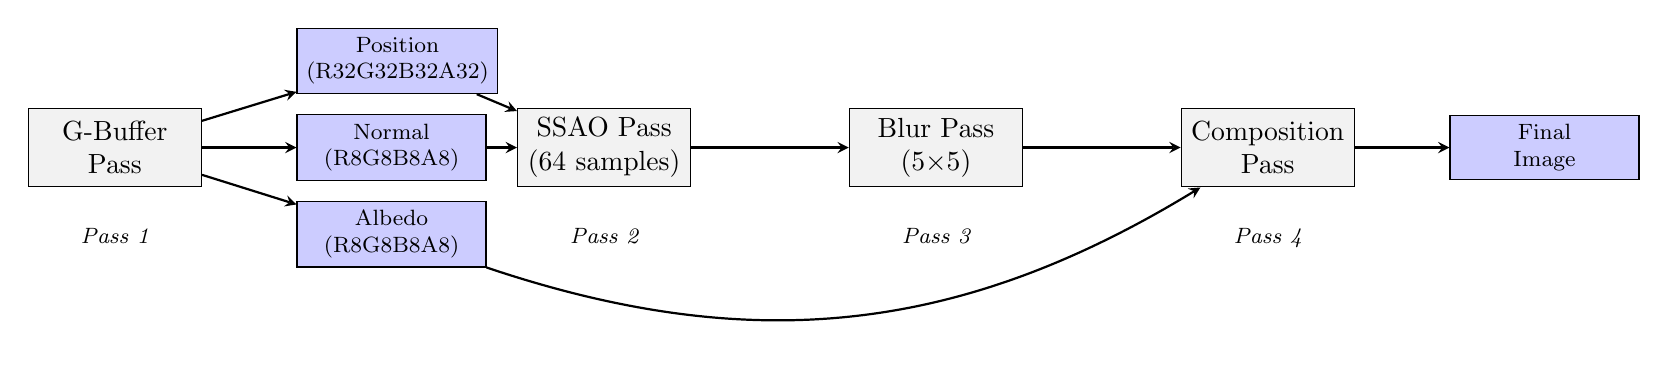
\begin{tikzpicture}[
            node distance=1.5cm,
            box/.style={rectangle, draw, minimum width=2.2cm, minimum height=1cm, align=center, fill=gray!10},
            data/.style={rectangle, draw, minimum width=2.4cm, minimum height=0.8cm, align=center, fill=blue!20, font=\footnotesize},
            arrow/.style={->, thick, >=stealth}
        ]
            % Pass 1
            \node[box] (gbuffer) {G-Buffer\\Pass};
            \node[data, right=1.2cm of gbuffer, yshift=1.1cm] (pos) {Position\\(R32G32B32A32)};
            \node[data, right=1.2cm of gbuffer] (norm) {Normal\\(R8G8B8A8)};
            \node[data, right=1.2cm of gbuffer, yshift=-1.1cm] (alb) {Albedo\\(R8G8B8A8)};

            % Pass 2
            \node[box, right=4cm of gbuffer] (ssao) {SSAO Pass\\(64 samples)};

            % Pass 3
            \node[box, right=2cm of ssao] (blur) {Blur Pass\\(5$\times$5)};

            % Pass 4
            \node[box, right=2cm of blur] (comp) {Composition\\Pass};

            % Output
            \node[data, right=1.2cm of comp] (out) {Final\\Image};

            % Arrows
            \draw[arrow] (gbuffer) -- (pos);
            \draw[arrow] (gbuffer) -- (norm);
            \draw[arrow] (gbuffer) -- (alb);
            \draw[arrow] (pos) -- (ssao);
            \draw[arrow] (norm) -- (ssao);
            \draw[arrow] (ssao) -- (blur);
            \draw[arrow] (blur) -- (comp);
            \draw[arrow] (alb) to[bend right=25] (comp);
            \draw[arrow] (comp) -- (out);

            % Labels
            \node[below=0.4cm of gbuffer, font=\footnotesize\itshape] {Pass 1};
            \node[below=0.4cm of ssao, font=\footnotesize\itshape] {Pass 2};
            \node[below=0.4cm of blur, font=\footnotesize\itshape] {Pass 3};
            \node[below=0.4cm of comp, font=\footnotesize\itshape] {Pass 4};
        \end{tikzpicture}%
        }
        \caption{SSAO rendering pipeline architecture. The position buffer is sampled 64 times per pixel in Pass 2, making it the primary target for FP16 conversion.}
        \label{fig:ssao-pipeline}
    \end{figure}

    \subsubsection{Baseline Resource Usage}

    Table~\ref{tab:ssao-baseline} shows the original resource allocation at 1920$\times$1080 resolution. The position buffer dominates memory usage at 47\% of the total G-buffer allocation, consuming 33.75 MB at full FP32 precision. Combined with the fact that this buffer is sampled 64 times per pixel during the SSAO pass, it represents an attractive target for FP16 conversion with potential benefits in both memory footprint and bandwidth.

    \begin{table}[H]
        \centering
        \caption{SSAO baseline (FP32 position buffer) memory allocation at 1920$\times$1080}
        \label{tab:ssao-baseline}
        \begin{tabular}{llrr}
            \toprule
            \textbf{Buffer} & \textbf{Format} & \textbf{Bits/Pixel} & \textbf{Size (MB)} \\
            \midrule
            Position + Depth & R32G32B32A32\_SFLOAT & 128 & 33.75 \\
            Depth & D32\_SFLOAT & 32 & 16.88 \\
            Normal & R8G8B8A8\_UNORM & 32 & 8.44 \\
            Albedo & R8G8B8A8\_UNORM & 32 & 8.44 \\
            SSAO Output & R8\_UNORM & 8 & 2.11 \\
            SSAO Blur & R8\_UNORM & 8 & 2.11 \\
            \midrule
            \textbf{Total} & & & \textbf{71.72} \\
            \bottomrule
        \end{tabular}
    \end{table}

    \subsubsection{FP16 Conversion and Risk Assessment}

    The position buffer format was changed from \texttt{VK\_FORMAT\_R32G32B32A32\_SFLOAT} to \texttt{VK\_FORMAT\_R16G16B16A16\_SFLOAT}. No shader modifications were required as the Vulkan implementation handles format conversion automatically when writing to and reading from the attachment.

    Prior to implementation, the conversion risks were assessed. View-space positions in the test scene range from approximately $-10$ to $+10$ units, well within FP16's range of $\pm 65,504$. At magnitude 10, FP16 provides precision of approximately 0.01 units, which is sufficient for screen-space sampling where sub-pixel accuracy is not required. The SSAO algorithm itself samples relative positions and computes depth differences rather than relying on precise absolute values, meaning small errors in position are unlikely to affect the binary occlusion test that determines whether a sample is occluded.

    \subsubsection{Results}

    The benchmark results, summarized in Table~\ref{tab:ssao-results}, demonstrate significant improvements from the FP16 conversion. The frame rate increased from 265.30 FPS to 374.11 FPS, representing a 41\% performance improvement. Total GPU memory decreased from 71.72 MB to 54.84 MB, a reduction of 23.5\% overall and exactly 50\% for the position buffer itself.

    \begin{table}[H]
        \centering
        \caption{SSAO performance comparison: FP32 vs FP16 position buffer}
        \label{tab:ssao-results}
        \begin{tabular}{lrrr}
            \toprule
            \textbf{Metric} & \textbf{FP32 Baseline} & \textbf{FP16 Position} & \textbf{Change} \\
            \midrule
            Total Frames & 7,959 & 11,224 & +3,265 \\
            FPS & 265.30 & 374.11 & \textbf{+41.0\%} \\
            Avg Frame Time & 3.77 ms & 2.67 ms & $-1.10$ ms \\
            \midrule
            Total GPU Memory & 71.72 MB & 54.84 MB & \textbf{$-23.5\%$} \\
            Position Buffer & 33.75 MB & 16.88 MB & $-50.0\%$ \\
            \bottomrule
        \end{tabular}
    \end{table}

    The 41\% FPS improvement significantly exceeds what might be expected for a simple format change. Analysis suggests this amplified benefit comes from multiple factors working together. The SSAO pass samples the position buffer 64 times per pixel, so halving the buffer size halves the memory traffic for this bandwidth-intensive operation. The smaller buffer fits more data in L2 cache, reducing round-trips to VRAM. And reduced bandwidth pressure on the memory controller allows more parallel memory requests to be serviced.

    Image quality metrics, shown in Table~\ref{tab:ssao-quality}, confirm that the visual impact of FP16 conversion is imperceptible. The PSNR of 63.01 dB is well above the 50 dB threshold typically considered visually lossless, and the SSIM of 0.9998 indicates near-perfect preservation of structural features such as edges and textures. All 20 sampled frames across the benchmark showed identical quality metrics, demonstrating stable quality rather than occasional degradation.

    \begin{table}[H]
        \centering
        \caption{SSAO visual quality metrics (average of 20 frame samples)}
        \label{tab:ssao-quality}
        \begin{tabular}{lrl}
            \toprule
            \textbf{Metric} & \textbf{Value} & \textbf{Interpretation} \\
            \midrule
            MSE & 0.0325 & Virtually zero error \\
            PSNR & 63.01 dB & Visually lossless ($>50$ dB) \\
            SSIM & 0.9998 & Near-perfect structural similarity \\
            \bottomrule
        \end{tabular}
    \end{table}

    \subsubsection{Analysis}

    The SSAO case study demonstrates an ideal scenario for FP16 adoption. The values stored are bounded to a known range (view-space positions), the algorithm uses relative operations (position differences for depth comparison) rather than requiring precise absolute values, the buffer is sampled at a high rate (64 times per pixel) which amplifies bandwidth benefits, and the buffer contains intermediate data that is not directly viewed rather than final output.

% ============================================================================
    \section{Discussion}
    \label{sec:discussion}
% ============================================================================

    \subsection{Analysis of Results}
    \label{subsec:cross-analysis}

    The SSAO case study provides strong evidence for the viability of hybrid precision rendering, with the 41\% performance improvement and 23.5\% memory reduction achieved with imperceptible quality loss demonstrating that significant optimizations are achievable through careful format selection.

    The magnitude of the performance improvement deserves particular attention. A naive expectation might be that halving a buffer's size would improve performance by at most a few percent, as modern GPUs have substantial memory bandwidth and caching capabilities.

    However, the 41\% improvement reflects the multiplicative nature of bandwidth reduction in sampling-intensive algorithms: when a buffer is read 64 times per pixel across millions of pixels, even small per-sample savings compound into large aggregate benefits. This has implications for similar techniques such as screen-space reflections, volumetric lighting, HBAO, and GTAO.

    The candidate selection analysis revealed an interesting pattern in existing practice. The Vulkan Examples' deferred rendering implementation already uses \texttt{R16G16B16A16\_SFLOAT} for position and normal G-buffers, indicating that experienced graphics programmers have independently recognized FP16 as appropriate for these use cases. The bloom example's use of \texttt{R8G8B8A8\_UNORM} at small resolution demonstrates that even lower precision can be acceptable when the visual requirements permit. These findings suggest that FP16 adoption for G-buffer data is not novel but rather represents a best practice that is sometimes overlooked.

    \subsection{Practical Guidelines}
    \label{subsec:guidelines}

    Based on the analysis conducted in this study, several guidelines emerge for developers:

    \textbf{Target view-space G-buffers first.} Positions and normals represent low-risk, high-reward targets for FP16 conversion. The bounded coordinate ranges and relative nature of common algorithms align well with FP16's characteristics. World-space buffers require more caution due to potentially larger coordinate ranges.

    \textbf{Profile before optimizing.} Not all formats benefit equally. Using tools like RenderDoc or NVIDIA Nsight to identify bandwidth-bound passes helps target optimization effort. A 50\% reduction in one buffer may yield minimal or substantial improvement depending on whether that buffer is the actual bottleneck.

    \textbf{Measure quality objectively.} Implementing automated measurement with metrics like PSNR and SSIM is preferable to visual inspection alone. The human eye can miss subtle degradation, and consistent automated testing provides confidence that edge cases are covered.

    \textbf{Test extreme scenarios.} Include unusual camera positions, bright light sources, and configurations that stress FP16's precision limits. Production applications should verify behavior across their full content range.

    \textbf{Consider portability.} When supporting hardware with different FP16 capabilities, flexible precision types like \texttt{min16float} provide a conservative approach that gains benefits where available while falling back gracefully.

    \subsection{Future Work}
    \label{subsec:future}

    Several directions merit further investigation:
    \begin{itemize}
        \item \textbf{Additional case studies:} Shadow mapping, screen-space reflections, and volumetric rendering could expand the catalog of FP16-appropriate use cases
        \item \textbf{Shader arithmetic precision:} Beyond buffer formats, the \texttt{mediump} qualifier may provide additional gains on mobile GPUs
        \item \textbf{Hybrid HDR pipelines:} Using FP16 for intermediate calculations with FP32 accumulators could balance precision and performance
        \item \textbf{Cooperative vector integration:} As the technology matures, integration of small neural networks for learned denoising or neural material evaluation represents an emerging frontier
    \end{itemize}

% ============================================================================
    \section{Conclusion}
    \label{sec:conclusion}
% ============================================================================

    This paper has investigated hybrid FP16/FP32 precision in real-time graphics pipelines through analysis of floating-point fundamentals, hardware capabilities, emerging technologies, and experimental case studies.

    \textbf{Key findings from the SSAO case study:}
    \begin{itemize}
        \item 41\% performance improvement from a single buffer format change
        \item 23.5\% memory reduction (50\% for the position buffer)
        \item Quality preserved at imperceptible levels (PSNR 63~dB, SSIM 0.9998)
        \item Performance exceeded expectations, indicating bandwidth as the limiting factor
    \end{itemize}

    \textbf{Selection matters:} View-space positions, normals, and similar bounded intermediate data are ideal candidates for FP16 conversion, while final output buffers and small allocations offer less opportunity. The finding that established Vulkan examples already use FP16 for G-buffers validates that experienced developers recognize these optimization opportunities.

    \textbf{Future directions:} Cooperative matrices and cooperative vectors offer additional potential but are currently most applicable to neural network inference. For traditional pipelines, hybrid FP16/FP32 precision represents a practical, low-risk technique that can deliver substantial improvements when applied with appropriate analysis of value ranges and precision requirements combined with objective quality measurement.

% ============================================================================
% References
% ============================================================================
    \bibliographystyle{plain}
    \begin{thebibliography}{99}

        \bibitem{ieee754}
        IEEE Computer Society. \textit{IEEE Standard for Floating-Point Arithmetic}. IEEE Std 754-2019, 2019.

        \bibitem{mjp-fp16}
        M. Pettineo. ``Shader FP16.'' The Danger Zone Blog, 2024.
        Available: \url{https://therealmjp.github.io/posts/shader-fp16/}

        \bibitem{vk-coop-matrix}
        Khronos Group. ``VK\_KHR\_cooperative\_matrix.'' Vulkan Documentation, 2023.
        Available: \url{https://docs.vulkan.org/features/latest/features/proposals/VK_KHR_cooperative_matrix.html}

        \bibitem{vk-coop-vector}
        Khronos Group. ``VK\_NV\_cooperative\_vector.'' Vulkan Documentation, 2024.
        Available: \url{https://docs.vulkan.org/features/latest/features/proposals/VK_NV_cooperative_vector.html}

        \bibitem{nvidia-coop-matrix}
        J. Bolz and J. Barczak. ``Machine Learning Acceleration in Vulkan with Cooperative Matrices.'' NVIDIA Developer Blog, 2019.
        Available: \url{https://developer.nvidia.com/blog/machine-learning-acceleration-vulkan-cooperative-matrices/}

        \bibitem{nvidia-neural-rendering}
        NVIDIA. ``Neural Rendering in NVIDIA OptiX Using Cooperative Vectors.'' NVIDIA Developer Blog, 2024.
        Available: \url{https://developer.nvidia.com/blog/neural-rendering-in-nvidia-optix-using-cooperative-vectors/}

        \bibitem{dx-coop-vector}
        Microsoft. ``Enabling Neural Rendering in DirectX: Cooperative Vector Support Coming Soon.'' DirectX Developer Blog, 2024.
        Available: \url{https://devblogs.microsoft.com/directx/enabling-neural-rendering-in-directx-cooperative-vector-support-coming-soon/}

        \bibitem{nrc-nvidia}
        T. M\"uller, F. Rousselle, J. Nov\'ak, and A. Keller. ``Real-time Neural Radiance Caching for Path Tracing.'' \textit{ACM Transactions on Graphics (SIGGRAPH)}, 40(4), 2021.

        \bibitem{vk-examples}
        S. Willems. ``Vulkan C++ Examples and Demos.'' GitHub Repository.
        Available: \url{https://github.com/SaschaWillems/Vulkan}

        \bibitem{ssao-crytek}
        M. Mittring. ``Finding Next Gen: CryEngine 2.'' \textit{SIGGRAPH 2007 Course: Advanced Real-Time Rendering in 3D Graphics and Games}, 2007.

        \bibitem{learnopengl-ssao}
        J. de Vries. ``SSAO.'' LearnOpenGL.
        Available: \url{https://learnopengl.com/Advanced-Lighting/SSAO}

        \bibitem{nvidia-tensor}
        NVIDIA. ``NVIDIA Ada Lovelace Architecture Whitepaper.'' NVIDIA, 2022.

        \bibitem{fp16-wiki}
        Wikipedia contributors. ``Half-precision floating-point format.'' Wikipedia, The Free Encyclopedia.
        Available: \url{https://en.wikipedia.org/wiki/Half-precision_floating-point_format}

    \end{thebibliography}

\end{document}
